%%%%%%%%%%%%%%%%%%%%%%%%%%%%%% -*- Mode: Latex -*- %%%%%%%%%%%%%%%%%%%%%%%%%%%%
%% uhtest.tex -- 
%% Author          : Robert Brewer
%% Created On      : Wed Sep 30 16:08:49 1998
%% Last Modified By: Robert Brewer
%% Last Modified On: Mon Oct  5 16:17:16 1998
%% RCS: $Id: uhtest.tex,v 1.2 1998/10/06 02:04:56 rbrewer Exp rbrewer $
%%%%%%%%%%%%%%%%%%%%%%%%%%%%%%%%%%%%%%%%%%%%%%%%%%%%%%%%%%%%%%%%%%%%%%%%%%%%%%%
%%   Copyright (C) 1998 Robert Brewer
%%%%%%%%%%%%%%%%%%%%%%%%%%%%%%%%%%%%%%%%%%%%%%%%%%%%%%%%%%%%%%%%%%%%%%%%%%%%%%%

%!!!!!!!!!!!!!!!!!!!!!!!!!!!!!!!!!!!!!!!!!!!!!!!!!!!!!!!!!!!!!!!!!!!!!!!!!!!!!!
%!NOTE: This example file has been prepared according to the University of
%!      Hawaii Style & Policy Manual for Theses and Dissertations dated
%!      "Revised February 1998". If you have one with a later date, you may
%!      need to make revisions to this document as well. In any event, making
%!      sure your thesis complies with Graduate Division guidelines is
%!      ultimately your responsibility. Caveat LaTeXtor. :)
%!!!!!!!!!!!!!!!!!!!!!!!!!!!!!!!!!!!!!!!!!!!!!!!!!!!!!!!!!!!!!!!!!!!!!!!!!!!!!!

%% The options are (you can only choose one from each group):
%%
%% 10pt, 11pt, 12pt: chooses the point size for the document. "11pt" is the
%%                   default.
%%
%% oneside, twoside: whether you want your document onesided or twosided. Note
%%                   that twosided is not guaranteed to work, and style
%%                   guidelines prohibit double sided printouts on final
%%                   copy. "oneside" is the default.
%%
%% draft, final: when printing drafts you can save a lot of paper by using the
%%               "draft" option. It switches to single spacing, displays overful
%%               hboxes with a black box, prints a version number on title page 
%%               and omits signature page. Of course for the final copy make
%%               sure to use the "final" option! "final" is the default.
%%
%% cm, times, palatino, newcent, bookman: switches between different font
%%                                        sets. "cm" is the Computer Modern
%%                                        font (TeX's default), the rest are
%%                                        PostScript fonts. "times" is the
%%                                        default.
%%
%% thesis, dissertation: switches between the style for a master's thesis and a 
%%                       Ph.D. dissertation. The differences are fairly minor
%%                       and limited to the front matter. "thesis" is the
%%                       default.
%%
%% actual, proposal: switches between actual document and proposal mode. In
%%                   proposal mode: the title page is simplified, the
%%                   version number is always printed, and the signature page
%%                   is omitted.
%%
%%% Load the uhthesis2e document class
\documentclass[11pt,final,times,dissertation,proposal]{uhthesis2e}

%%% Load some useful packages:
%% New LaTeX2e graphics support
\usepackage{graphicx}
%%	using final option to force graphics to be included even in draft mode
%\usepackage[final]{graphicx}
%% Tell graphicx the default directory for all figures
\graphicspath{{figures/final/}}

%% Enable subfigure support
\usepackage{subfigure}

%% Make subsubsections numbered and included in ToC
\setcounter{secnumdepth}{3}
\setcounter{tocdepth}{3}

%% Package to linebreak URLs in a sane manner.
\usepackage{url}

%% Define a new 'smallurl' style for the package that will use a smaller font.
\makeatletter
\def\url@smallurlstyle{%
  \@ifundefined{selectfont}{\def\UrlFont{\sf}}{\def\UrlFont{\small\ttfamily}}}
\makeatother
%% Now actually use the newly defined style.
\urlstyle{smallurl}

%% Define 'tinyurl' style for even smaller URLs (such as in tables)
\makeatletter
\def\url@tinyurlstyle{%
  \@ifundefined{selectfont}{\def\UrlFont{\sf}}{\def\UrlFont{\scriptsize\ttfamily}}}
\makeatother

%% Puts space after macros, unless followed by punctuation
\usepackage{xspace}

%%% Personal macros
%% Tired of typing CO2 so many times, requires xspace package
\newcommand{\COtwo}{CO\ensuremath{_2}\xspace}

%% Allows insertion of fixme notes for future work
\usepackage[footnote, nomargin]{fixme}

%% Make URLs clickable
\usepackage[colorlinks, bookmarks=false]{hyperref}
%\usepackage[colorlinks, bookmarks=true]{hyperref}

%% Make links to captions point to the figure, not just the caption at bottom
\usepackage[all]{hypcap}

%% Since I'm using the LaTeX Makefile that uses dvips, I need this
%% package to make URLs break nicely
\usepackage{breakurl}

%%% End of preamble
\begin{document}

%%% Declarations for Front Matter. Capitalize all of these values
%%% "normally". This allows the document class to format them properly.
%% Full title of thesis or dissertation, capitalized like a title should be.
\title{Carbon Metric Collection and Analysis with the Personal Environmental
Tracker or Something}
%% Your name, capitalized normally. Do not include any titles like Dr.
\author{Robert S. Brewer}
%% Month in which you intend to receive your degree (i.e. graduation).
%% Presumably this will be one of: May, August, or December.
\degreemonth{May}
%% Year of expected graduation.
\degreeyear{2009}
%% Type of degree to be conferred.
\degree{Doctor of Philosophy}
%% This is the chairperson of your committee. Do not use titles like Dr.
\chair{Philip M. Johnson}
%% The other members of your committee, seperated by "\\". Again, no titles,
%% and it is customary to list the outside committee member (if you have one)
%% last.
\othermembers{Foo Bar\\
Baz Biff\\
Joseph B. Bogus\\
Otto O. Outsider}
%% This is the total size of your committee, including the chairperson. The
%% signature page routine will only handle up to 6 members; if you have more
%% than that you will need to modify the document class.
\numberofmembers{5}
%% The field in which you are obtaining your degree, capitalized normally.
\field{Computer Science}
%% The version number of your document. Consistent use of this will enable you
%% to tell old drafts from new ones. Final actual documents omit this
%% automatically so you can use it without fear of submission problems at the
%% end. If you do not define this parameter, it defaults to "1.0.0".
\versionnum{0.2.0}

%%% Create the title page from all the information above. Note that the
%%% titlepage is outside the front matter.
\maketitle

\begin{frontmatter}

%%% Create the signature page (when indicated by the options)
\signaturepage

%%% Create the copyright page
%\copyrightpage

%%% Bring in the dedication page from external file
%%%%%%%%%%%%%%%%%%%%%%%%%%%%%%% -*- Mode: Latex -*- %%%%%%%%%%%%%%%%%%%%%%%%%%%%
%% uhtest-dedication.tex -- 
%% Author          : Robert Brewer
%% Created On      : Fri Oct  2 16:29:01 1998
%% Last Modified By: Robert Brewer
%% Last Modified On: Fri Oct  2 16:29:20 1998
%% RCS: $Id: uhtest-dedication.tex,v 1.1 1998/10/06 02:07:25 rbrewer Exp $
%%%%%%%%%%%%%%%%%%%%%%%%%%%%%%%%%%%%%%%%%%%%%%%%%%%%%%%%%%%%%%%%%%%%%%%%%%%%%%%
%%   Copyright (C) 1998 Robert Brewer
%%%%%%%%%%%%%%%%%%%%%%%%%%%%%%%%%%%%%%%%%%%%%%%%%%%%%%%%%%%%%%%%%%%%%%%%%%%%%%%
%% 

\begin{dedication}
\null\vfil
{\large
\begin{center}
To myself,\\\vspace{12pt}
Perry H. Disdainful,\\\vspace{12pt}
the only person worthy of my company.
\end{center}}
\vfil\null
\end{dedication}


%%% Bring in the acknowledgements section from external file
%%%%%%%%%%%%%%%%%%%%%%%%%%%%%%% -*- Mode: Latex -*- %%%%%%%%%%%%%%%%%%%%%%%%%%%%
%% uhtest-acknowledgements.tex -- 
%% Author          : Robert Brewer
%% Created On      : Fri Oct  2 16:29:43 1998
%% Last Modified By: Robert Brewer
%% Last Modified On: Fri Oct  2 16:29:52 1998
%% RCS: $Id: uhtest-acknowledgements.tex,v 1.1 1998/10/06 02:06:54 rbrewer Exp $
%%%%%%%%%%%%%%%%%%%%%%%%%%%%%%%%%%%%%%%%%%%%%%%%%%%%%%%%%%%%%%%%%%%%%%%%%%%%%%%
%%   Copyright (C) 1998 Robert Brewer
%%%%%%%%%%%%%%%%%%%%%%%%%%%%%%%%%%%%%%%%%%%%%%%%%%%%%%%%%%%%%%%%%%%%%%%%%%%%%%%
%% 

\begin{acknowledgements}
I want to ``thank'' my committee, without whose ridiculous demands, I
would have graduated so, so, very much faster.
\end{acknowledgements}


%%% Bring in the abstract section from external file
%%%%%%%%%%%%%%%%%%%%%%%%%%%%%% -*- Mode: Latex -*- %%%%%%%%%%%%%%%%%%%%%%%%%%%%
%% uhtest-abstract.tex -- 
%% Author          : Robert Brewer
%% Created On      : Fri Oct  2 16:30:18 1998
%% Last Modified By: Robert Brewer
%% Last Modified On: Fri Oct  2 16:30:25 1998
%% RCS: $Id: uhtest-abstract.tex,v 1.1 1998/10/06 02:06:30 rbrewer Exp $
%%%%%%%%%%%%%%%%%%%%%%%%%%%%%%%%%%%%%%%%%%%%%%%%%%%%%%%%%%%%%%%%%%%%%%%%%%%%%%%
%%   Copyright (C) 1998 Robert Brewer
%%%%%%%%%%%%%%%%%%%%%%%%%%%%%%%%%%%%%%%%%%%%%%%%%%%%%%%%%%%%%%%%%%%%%%%%%%%%%%%
%% 

\begin{abstract}
Abstract goes here, and will be written once the proposal is mostly done.
\end{abstract}


%%% Generate table of contents
\tableofcontents

%%% Generate list of tables
\listoftables

%%% Generate list of figures
\listoffigures

\end{frontmatter}

%%% Bring in the body of the thesis from external file
%%%%%%%%%%%%%%%%%%%%%%%%%%%%%%% -*- Mode: Latex -*- %%%%%%%%%%%%%%%%%%%%%%%%%%%%
%% proposal-body.tex -- 
%% Author          : Robert Brewer
%% Created On      : Fri Sep  5 13:50:18 1997
%% Last Modified By: Robert Brewer
%% Last Modified On: Fri Sep 18 15:01:09 1998
%% RCS: $Id: proposal-body.tex,v 1.3 1998/09/19 00:29:24 rbrewer Exp rbrewer $
%%%%%%%%%%%%%%%%%%%%%%%%%%%%%%%%%%%%%%%%%%%%%%%%%%%%%%%%%%%%%%%%%%%%%%%%%%%%%%%
%%   Copyright (C) 1998 Robert Brewer
%%%%%%%%%%%%%%%%%%%%%%%%%%%%%%%%%%%%%%%%%%%%%%%%%%%%%%%%%%%%%%%%%%%%%%%%%%%%%%%
%% 

\chapter{Introduction}

\section{The Problem with Mailing List Archives}
Electronic mailing lists provide an excellent way for people to rapidly share
information on a specific topic. In some cases the topic is extremely focused
and highly technical, thereby providing a resource which cannot be found
outside of the electronic realm. Many mailing lists store the messages sent to
the list in an archive for future retrieval. These archives can range from
giant text files to databases with sophisticated WWW interfaces. The two most
common types of archives are:
\begin{itemize}
\item browsable thread-based archives that allow a user to read messages in a
  format similar to the one in which they were sent to the list
\item searchable archives that allow users to do full-text searches over all
  the articles in the archive.
\end{itemize}

The mailing list format has a few important benefits: it is intuitively easy to
participate, software required to participate is widely available, and it makes
use of widely deployed server-support (many mail servers have mailing list
distribution functionality). Unfortunately these very benefits prevent the
fullest use of the information in the mailing list data stream.  Since anyone
can contribute to the list and the format is very conversation-like, the result
is a data stream with a mediocre signal to noise ratio at best. While there is
a lot of valuable knowledge available, one has to slog through endless newbie
questions, flamewars, and ``Me Too''s.

The problem becomes even worse when you take into account the archives of the
list. When users consult a mailing list archive, they often are searching for
a specific piece of information like a solution to a problem they are having.
Unfortunately mailing list archives are poorly equipped to support that kind of
query. All the irrelevant information that was sent to the list is immortalized
in the archive, making it difficult to find the useful information. Searchable
archives also face the problem that any particular query may return an enormous
number of hits. For example, a search for ``OSPF'' (Open Shortest Path First, a
modern TCP/IP routing protocol) on the ascend-users mailing list archive
\cite{nexial-ascend-website} returns 650 hits which is an artificially imposed
maximum. In this case the hits are displayed in reverse chronological order,
which isn't necessarily desirable if you are looking for a particular OSPF
problem.

Some mailing list communities generate a list of Frequently Asked Questions
(FAQs) for the mailing list. Originally the purpose of a FAQ was to avoid the
recurring situation where new subscribers to the list would ask questions that
had been asked and answered many times before. By creating a list of these
frequently asked questions, it was hoped that newbies would read the FAQ and
have their questions answered that way. The FAQ format is also used as a
convenient format for disseminating useful information on the subject matter,
i.e., questions that might not be frequently asked but are useful to know. The
big problem with FAQs is that they are primarily maintained by hand. This means
that keeping an FAQ up to date is a labor-intensive process which frequently
exhausts the volunteer maintainer. FAQs are generally intended to be documents
(text, HTML, etc.) which can the distributed (posted to a newsgroup, downloaded
from a web page). This ``distributable'' quality limits the size and
organization of the document to something that can be read and understood by a
human. The combination of these two factors limits the amount and depth of
information that can be presented; in other words an FAQ almost by definition
leaves out useful information if it isn't used frequently enough to justify its
inclusion to the space-limited FAQ. An additional failing of FAQs is that they
are not designed to deal with questions whose answer frequently changes. The
answer to a question like ``What is the most stable firmware version supporting
frame relay?'' may change from week to week as new firmware releases are
released. Answering this question would require frequent revisions and put
excessive demands on the FAQ maintainer.

\section{Condensation as a Solution}
To solve the problems inherent in current mailing list archives, I propose a
process called {\em condensation} whereby one can strip out all the extraneous,
conversational aspects of the data stream leaving only the pearls of
interconnected wisdom. This condensation takes the voluminous data stream from
the mailing list and extracts the useful information. As an analogy, newspapers
provide a daily report on current events, but their analysis of which events
are accurate or relevant are limited in that newspapers have short deadlines, a
broad subscriber base, and other considerations. A story published one day
might be amended or retracted the next depending on how events unfold.
However, a book describing world events will tend to have a longer deadline
which permits more reflection and analysis: a hoax which might occupy weeks of
headlines in a newspaper will probably be little more than a footnote in a book
(unless the book is about newspaper hoaxes). It is this refinement of
information that I refer to as condensation.

There are a variety of ways that the information could be condensed, depending
on the intended use of the archive. Our goal is to provide a searchable archive
of information that allows archive users to quickly find answers to specific
queries (see Section \ref{sec:op-scenarios}). Since the goal is to respond to
user queries, preserving the threaded nature of the mailing list is not
relevant.  Condensation will require omitting unimportant messages, removing
unimportant portions of messages, inserting new text into messages when
required for clarification, and adding new messages to the database when that
is the best way to explain something. In order to support searching of the
archive, messages will be assigned a type and annotated with keywords. A
condensed archive will not suffer from the problems of an unabridged searchable
archive. Since only truly useful information will be put into the archive, the
amount of data to be searched is smaller which improves the odds of a search
being accurate. Also, since condensation uses a set of standardized keywords a
user can be sure that messages using different terms but discussing the same
topic will be retrieved by a search. Condensation also solves the problems
facing FAQs. Since condensation relies on a centralized archive, it does not
face the same size and complexity constraints that an FAQ does. The issue
raised earlier with FAQs about questions whose answer changes frequently are
handled well by a condensed archive, where the answer to a question can be a
query to the archive database. Each time the answer is requested, it can be
constructed from the latest information input into the condensed archive.

\section{MCS: A System For Condensation}
To explore this idea of mailing list condensation and to test whether or not a
condensed archive of a mailing list is actually better than traditional
archives, I propose the construction and evaluation of a new software system.
I name this system (for lack of imagination) the Mailing list Condensation
System or MCS. MCS will have two main parts: one which is dedicated to taking
the raw material from the mailing list and condensing it, and another which
stores the condensed messages and allows users to retrieve them.

One way to perform the condensation would be to implement an AI system that
reads the messages and then decides what information keep, what to throw away,
and what keywords to assign to each. In order to perform this task adequately,
the system would need superb natural language processing capabilities and an
in-depth knowledge of the mailing list domain. I believe the implementation of
such a system is infeasible. If possible, it would require substantial
expenditure of resources to complete.

As an alternative to an AI approach, I propose that this process of
condensation be carried out by a human editor with the help of software tool.
Humans are quite good at examining textual information and determining what is
useful and what is not, while computers are good at queries across structured
data \cite{Brooks:1996:CST}. It will also be far more resource efficient
because most mailing lists already have a set of `gurus'; subscribers who read
all messages sent to the list and who are domain experts.  Therefore in MCS
humans will do the editing using the MCS editing program which will make the
process as efficient as possible. Only the editors will need to use the editing
program.

The storage and retrieval portion of MCS will consist of a web server connected
to a database system. As editors create condensed messages, they will be placed
into the database by the editing program. For ease of use, end-users will
access the condensed archive with a web browser. The MCS-generated web site
will provide a variety of forms or applets which will allow users to browse or
query the database.

\section{An Example}
\label{sec:example}
To show how condensation can create a more useful archive than traditional
methods, I will consider an example query and show the results from
existing archives. Then I explain how a condensed archive would be different.

\subsection{The Question}
The example I have chosen is somewhat complicated and involves compiling and
installing perl 5.004\_04 on BSD/OS. Perl is a interpreted language which is
designed for text processing \cite{programming-perl}. BSD/OS is an operating
system from Berkeley Software Design Inc. (BSDI) which runs on Intel-based
computers \cite{bsd-os}. BSD/OS has a user-maintained mailing list called
``bsdi-users'' for discussion of all issues about the operating system. For
this example I will use the actual information available from the
``bsdi-users'' mailing list.

Perl 5.004\_04 comes with an automated configuration program which configures
and compiles the software when told what operating system it is running on.
Unfortunately, there is a problem with the configuration script. When this
version of perl was released, BSDI was working on a new version of BSD/OS. At
that time, the new version was assigned number ``3.1''. The configuration
script for perl was set up so that certain changes would be made if perl was
installed on a 3.1 system. This would allow the same perl distribution to work
both on the existing 3.0 system and the new 3.1 system when it was released.
Unfortunately, the version which was to be called 3.1 was delayed and therefore
renumbered ``4.0''. A minor revision of BSD/OS was released with the (now
unused) version number ``3.1''. As a result of this version number mix up,
installing perl 5.004\_04 on a BSD/OS 3.1 system would fail in strange ways due
to the failure of some of the configuration assumptions. User's confusion over
this was compounded by the existence of the special configuration information
for BSD/OS 3.1 in perl: since perl had configuration information preset for
3.1, surely it couldn't be wrong?

This problem has three interesting attributes:
\begin{enumerate}
\item The solution to the problem is fairly simple: a single configuration
  script in the perl distribution needs to have all instances of ``3.1''
  changed to ``4.0'' and some other minor chances. The changes can either be
  made automatically through the Unix {\tt patch} command or be made by hand
  (once you understand the cause of the problem).
\item The problem has obvious symptoms which definitively indicate the problem:
  inability to install perl on BSD/OS 3.1 or specific error messages that occur
  when attempting to compile perl with unpatched configuration files.
\item The perl distribution is updated with bug fixes only infrequently so this
  problem was encountered by many people over several months. This caused
  people to post messages to bsdi-users asking for help with the same problem
  over and over again.
  \label{enum:repost}
\end{enumerate}

There are three well-known information sources related to or derived from the
bsdi-users mailing list: the BSD/OS FAQ, the Support Net archive, and the
Nexial Systems archive. I attempted to find the solution to the problem in
each information resource.

\subsection{The BSD/OS FAQ}
The BSD/OS FAQ \cite{bsdi-FAQ} is maintained by a single person as a volunteer
effort. There are 73 question/answer pairs in the FAQ, and it is not
immediately clear what method was used to order them. It appears
semi-chronological, but not completely. In any case, the word ``perl'' does not
appear in version 1.1.0 (dated 98/08/05 [sic]) and there is no discussion of
our example problem. It is possible that the question was in the FAQ at one
point and then later removed when the perl distribution was fixed, but this
seems unlikely given that there are other question/answer pairs in the FAQ
which are two years out of date. The fact that it is not in the FAQ is not
surprising. The FAQ is maintained in someone's spare time, so many useful
question/answer pairs will never make it in due to time constraints. The FAQ is 
also a manageable size at about 36 kilobytes, allowing it to be posted to the
mailing list on occasion. If the FAQ were to contain information every
installation problem for every package used with BSD/OS, it would probably grow 
unmanageable.

\subsection{The Support Net Archive}
The Support Net archive contains all messages posted to the mailing list over
the last 12 months \cite{supportnet-bsdi}. The messages are accessible in two
ways: each month's messages displayed in a thread format, or searched using the
Excite for Web Servers search engine (EWS) \cite{ews-website}. An example of
the thread format is shown in figure \ref{fig:supportnet-thread}. The thread
format is useful when trying to follow the flow of a conversation, but it is
ill-suited to finding a particular piece of information.

\begin{figure}[htbp]
  {\centerline {\psfig{figure=figs/supportnet-thread.eps}}}
%  {\centerline \includegraphics{figs/software-contents.eps}}
  \caption{Support Net bsdi-users archive viewed by thread}
  \label{fig:supportnet-thread}
\end{figure}

The EWS search engine used by Support Net indexes a collection of documents and
provides a ``concept-based architecture'' for searching. It claims to analyze
the document collection and determine ``statistical correlations between terms
and documents'' which improves recall and precision compared to other search
methods. In an attempt to find the answer to our example question, I performed
a search with input ``installing perl5 compile problems''. Part of the results
can be seen in figure \ref{fig:supportnet-search}.

\begin{figure}[htbp]
  {\centerline {\psfig{figure=figs/supportnet-search.eps}}}
%  {\centerline \includegraphics{figs/software-contents.eps}}
  \caption{Support Net bsdi-users archive search results}
  \label{fig:supportnet-search}
\end{figure}

The initial search returned a few relevant messages, but they were all written
by people who had encountered the problem and were asking for a solution. Using
the EWS query-by-example feature, I used one of these requests as the basis
for our new query. This resulted in several more messages asking for help on
the problem, and a few misguided attempts to help. Again, I selected the
message that best reflected the problem and performed a query-by-example. The
next batch of messages included one which acknowledged the problem, but
referred the person asking the question to the archives for the actual patch to
solve the problem! After fifteen minutes and several more iterations of
query-by-example, I obtained both a message containing the actual patch and a
message from BSDI personnel explaining the problem's genesis (as previously
summarized).

These results plainly show the problems with a traditional archive. Since every
message is included in the archive, messages repeating the question are often
returned by the search. Since the results are frequently sorted first by
relevance and then by date, these repeat questions are actually more likely to
be returned by a search than the first time the question was asked. The
repeated posting of questions also reduces the likelihood that a useful
response will be given, as evidenced by the ``look it up in the archives''
response and several repeats which did not appear to be answered at all. One
message responding to a repeat asks that the question/answer pair be put in the
FAQ, which we know has not been done! This shows that even though there was a
recognized need for this problem to be documented in the FAQ, it never happened
(for whatever reason).

\subsection{The Nexial Systems Archive}
The Nexial Systems archive provides a ``fuzzy'' search mechanism for the
bsdi-users list \cite{nexial-bsdi}. The fuzziness allows the engine to find
messages that match keywords that are spelled in a similar manner to the ones
provided by the user. Starting with the same initial set of keywords as the
search of the Support Net archives, I attempted to find the solution in the
Nexial archives. Finding the answer in the Nexial archive took longer and
required more effort because it does not provide a query-by-example facility.
This required `massaging' the keywords until I found ones that matched the
message containing the patch. Getting the keywords right also required us to
extract keywords from some of the earlier search results, like the word
``hint'' which refers to the hint file used by the configuration system which
the patch applies to.

The problems with traditional archives are the same in the Nexial archive. Most 
of the messages retrieved were users re-asking the question or answers which
just say ``consult the archives''. This latter request is somewhat amusing
considering that it is rather difficult to dig up the patch from either archive 
even when you know exactly what you are looking for. Another interesting point
is that the cycle of re-asking the question and being referred to the archives
is actually a feedback loop. Each time someone asks this question, they
increase the number of useless matches the next person querying the archives
will get. When someone cannot find the answer in the archives, the obvious
alternative is to post the question to the list {\em again}.

\subsection{The MCS Archive}
\label{sec:mcs-symptom-example}
There are several ways in which an MCS archive could be used to address the
example question. First and foremost, the MCS archive would only contain the
original message which contained the question, and a couple of responses (in
this case one containing the patch and one from BSDI which explains how the
problem came to be). This alone would dramatically reduce the effort required
to find the solution in the archive: since only the question and the canonical
answer are archived there are no extra messages to wade through. This lack of
repetition is assured by the editor who will either remember seeing this
problem before or consult the archive before adding new information to the
archive.

There are a variety of means by which a user can query the MCS archive. In the
case of the example question, the user would have access to error messages
produced by the compilation attempt like ``{\tt Invalid option `-fPIC'}''. This 
error message can be used as the symptom in MCS's symptom-based problem
lookup. Figure \ref{fig:mcs-symptomlookup} shows a mockup how a user would use
this type of query.

\begin{figure}[htbp]
  {\centerline {\psfig{figure=figs/mcs-symptomlookup.eps}}}
%  {\centerline \includegraphics{figs/software-contents.eps}}
  \caption{Mockup of MCS symptom-based problem lookup}
  \label{fig:mcs-symptomlookup}
\end{figure}

The results here show the ease with which the desired information is found.
Using the diagnostic error message, a list of problems which result in that
error message are displayed. Next to each problem are its known solutions,
which in the case of our example are the patch and the explanation. One can see
that the other problem with this symptom has only an explanation as a solution.

\section{Thesis Statement}
\label{sec:thesis-statement}
I believe that an MCS-generated mailing list archive maintained by an external
researcher will be adopted as a information resource by the subscribers of that
mailing list.  Furthermore, I believe that subscribers will prefer the
MCS-generated archive over existing traditional archives of the mailing list.

The traditional archives are any existing archives of a mailing list that allow 
either browsing of or searching through the messages posted to the list over
time. For example, in section \ref{sec:example} the traditional archives of the 
bsdi-users list are the Support Net and Nexial Systems archives.

I define adoption as a significant fraction of those using the traditional
archives of the list choosing to use the MCS archive either in addition or
instead of the traditional archives. Unfortunately, there is no straightforward
way to determine the number of people currently using traditional archives for
a list since I do not have control over those archives. Instead I plan to use
the number of list subscribers as an estimate of the number of potential MCS
users. The adoption percentage is then the number of MCS archive users divided
by the number of list subscribers, expressed as a percentage. For the purposes
of this research, I will consider an adoption percentage of 10\% or higher to
be indicative of success.

I define preference as the expression by users of the MCS archive that they
prefer to use the MCS archive when searching for information related to the
mailing list.

The caveat about maintenance by an external researcher is an important one.
Unlike traditional archives, an MCS archive requires effort to maintain its
usefulness. If someone not involved with this research was required to perform
the maintenance (thereby lacking an important motivator), adoption could be
much lower. For more discussion on this issue see chapter
\ref{cha:post-thesis}.


\chapter{System Specification}

\section{System Functionality}
The primary goal of MCS is to make life easier for users of electronic mailing
lists. It aims to take the messages sent to the list and transform them into an
archive of information which users can refer to when they have problems or
questions about the subject matter.

MCS will enable the maintainers of the archive to:
\begin{itemize}
\item Select messages for archival
\item Annotate each message with keywords from a standardized list
\item Add or delete text from the message for context or brevity
\item Link messages to one another
\end{itemize}

MCS will allow users of the archive to:
\begin{itemize}
\item Search for solutions to problems they are having
\item View tables of problem-reports which are organized by relevance
\item Browse through a list of important, time-sensitive messages
\end{itemize}

\section{Goals}

The primary goal of MCS is adoption by the user community. To encourage users
to adopt the system, there are two issues that MCS must be designed around.
Because MCS receives its input from a mailing list, it is crucial that MCS be
designed with the social structure of a user-supported mailing list in mind.
Specifically, the mailing list and its community should not be adversely
affected by MCS. Any attempt to impose restrictions on how people read or
participate in the list (like requiring users to use special software or
compose messages in a certain format) would be met with blistering criticism.
MCS must stand apart from the mailing list itself, resigned to using messages
from the list on an as-is basis.

MCS should also not attempt to condense all messages which come through the
list. If a user wants a comprehensive archive of all messages sent to the list,
he or she should be referred to an existing archive that serves that function.
The existence of other ``unabridged'' archives frees MCS to eliminate any
messages or parts of messages that are not worth archiving. It may be possible
to provide a link to the original article in an unabridged archive, for any
message in MCS which has been edited

\section{Target Mailing List}
To specify the requirements for the system, clearly I need to choose a
particular mailing list to target. I propose the ``ascend-users'' mailing
list, which is a user-created and user-administered list for the discussion of
the use and deployment of equipment produced by Ascend Communications
\cite{ascend-website}. Ascend Communications produces a wide array of
communications equipment with a primary focus on remote access (POTS dialup,
ISDN, frame relay, etc). One large segment of equipment users are Internet
Service Providers (ISPs) who provide Internet access to the public at large.

The ``ascend-users'' mailing list was chosen for the following reasons:

\begin{enumerate}
\item There mailing list is already archived in at least two locations, and the
  archives are well-used by the subscribers of the list.
\label{enu:choice-archives}

\item The topic of discussion is technical. The participants of the list use it
  primarily for information gathering on Ascend equipment and directly related
  topics (network topology, environmental controls for equipment rooms, etc).
  This list is not used for ``social'' purposes like chatting about current
  events or the weather. It will be easier to extract the ``useful''
  information from the list because there should be broad agreement as to which
  messages are considered useful, which might not be the case on a list with
  heavy social interaction.
\label{enu:choice-topic}

\item Most list subscribers are System Administrators (sysadmins).  Sysadmins
  are notoriously busy people. This fact works to our advantage for two
  reasons.  First, because they are short on free time, if they are willing to
  use a new system, (or data processed by a new system) that in itself will be
  an accomplishment. Second, they are likely to judge the system primarily by
  whether it helps them get their job done faster or not.
  
\item The topic of discussion is highly focused. The types of interaction on
  the list are fairly limited: requests for help troubleshooting a problem,
  answers to questions, real-world experiences with different software and
  hardware releases. This gives us leverage in what MCS can provide to users.
  For example, the stability and performance of different firmware patch
  releases is a topic of nearly constant discussion. Frequently a patch release
  will improve in some aspect (like performance), only to introduce new
  problems in other areas (like stability or security). It would be
  straightforward to provide a table of firmware versions and links to relevant
  discussion that occurred after their release.

\item The list is relatively low traffic. There are roughly 40-90 messages
  on the list a day, which should provide sufficient input to the condensation
  system without overwhelming the system or the maintainer of the system.
  
\item The author is highly familiar with the subject matter. The maintainer of
  the MCS archive will require knowledge of the mailing list topic in order to
  properly categorize information. The author can fill the role of maintainer
  because he is familiar with the mailing list and the equipment it discusses.
\end{enumerate}

Some of these reasons are really requirements for any list to be condensed by
MCS, and some are specific to the practicalities of this research project.
Requirement \ref{enu:choice-archives} applies to any list on which MCS is to be
used; obviously it makes no sense to create a condensed archive of a list if
nobody would ever wish to consult the archive!  Requirement
\ref{enu:choice-topic} also is important so that the editor need not spend a
great deal of time worrying over whether a message should be archived or not.
The rest of the reasons relate primarily to the evaluation of the system and
are therefore not requirements for future MCS targets.

It is also worth noting that ascend-users is hardly the only list which meets
the essential requirements. Several other lists like the previously mentioned
bsdi-users, portmaster-users, and the cisco mailing list
\cite{nexial-mailinglists} would be likely candidates for future adoption (see
chapter \ref{cha:post-thesis}).

\subsection{Classes of Users on ascend-users}
In order to better understand the mailing list, I have devised several
categories into which the subscribers to the ``ascend-users'' mailing list can
be divided. The categories are based on the subscriber's level of experience
with the equipment. Within each category, I will identify the goals that I
believe the group has with respect to their usage of the list (whether active
or passive).  I identify these goals so that one can see how a system might
meet some or all of their needs. The users have been categorized as:
prospective, newbie, intermediate, and advanced.

\subsubsection{Prospective User}
These subscribers have joined the list because they are interested in
determining whether they should use Ascend equipment. They currently neither
own nor directly manage Ascend equipment.

Objectives:
\begin{itemize}
\item Want to read the experiences of others using the equipment in a similar
  environment so they can decide whether to purchase Ascend equipment or not.
\item Want comparisons between Ascend and other comparable equipment.
\end{itemize}

\subsubsection{Newbie User (or just ``Newbie'')}
These subscribers have recently acquired or been put in charge of Ascend
equipment. They have little experience with the equipment, but they do have
ready access to it.

Objectives:
\begin{itemize}
\item Want step-by-step installation instructions for real-world configuration
  scenarios (ISP, corporate telecommuting, etc)
\item Want {\em brief} summary of information other subscribers think a newbie
  would find useful
\item Want glossary of frequently used terms
\item Want to know what firmware version to use
\item Want to know what equipment can do
\item Want to find quick answers to problems in configuration
\item Want pointers to more information
\end{itemize}

\subsubsection{Intermediate User}
These subscribers have been using Ascend equipment for more than three months
but less than twelve months. In general they have the equipment mostly working,
or they have at least spent considerable time trying to get it to work.

Objectives:
\begin{itemize}
\item Want to be able to browse through topics that have been brought up on the
  list
\item Want to find quick answers to operational problems
\item Want to be informed of new firmware releases
\item Want to be informed of hardware issues (recalls, new related products)
\end{itemize}

\subsubsection{Advanced User}
These subscribers have been using Ascend equipment for more than one year. They
are typically quite familiar with the equipment, and they have tuned their
configuration to meet their needs. Their needs are similar to the intermediate
user, with an addition.

Objectives:
\begin{itemize}
\item Want to be able to help others solve problems without having to read or
  answer the large volume of total questions posed to the list
\end{itemize}

\section{Operational Scenarios}
\label{sec:op-scenarios}
This section will provide several operational scenarios which describe ways in
which a user could potentially interact with MCS.

\subsection{Firmware Version Lore}
This is perhaps the most classic use of the ascend-users list. Every time a
firmware release for the Ascend MAX product line comes out people want to know
if it solves important long-standing problems, breaks existing configurations,
improves/degrades performance, etc. Some people are masochists (or are forced
to use the new version because of a show-stopping bug that affects them) and
try the new versions out right away, but most people take a wait-and-see
attitude. Also, people who have only recently acquired Ascend equipment (or a
particular model of Ascend equipment) want to know which version will best meet
their needs.

A very useful representation for the user would be a table of all existing
versions for a particular model. This table would have a link to the firmware
itself, a link to the Ascend release notes, and then a series of links to
whatever keywords appeared together with that version. For example, if there
are a lot of messages which discuss version 5.0Ap12 and its performance with
OSPF, then there should be a link on the table titled ``OSPF'' which takes you to
the appropriate messages. The table could also have a count of how many users
submitted positive or negative opinions on each version.

\begin{figure}[htbp]
  {\centerline {\psfig{figure=figs/software-contents.eps}}}
%  {\centerline \includegraphics{figs/software-contents.eps}}
  \caption{Software Contents Web Mockup}
  \label{fig:software-contents}
\end{figure}

\begin{figure}[htbp]
  {\centerline {\psfig{figure=figs/software-table.eps}}}
%  {\centerline \includegraphics{figs/software-contents.eps}}
  \caption{Software Table Web Mockup}
  \label{fig:software-table}
\end{figure}

\subsection{Hot Topics}
Many people subscribe to the mailing list but don't have time to keep up with
it most of the time. They just set their mailer to file messages from the list
into a folder and only look at it from time to time. However, it would be very
nice if one could see what topics are being discussed on the mailing list in
the last week or so. Scanning subject headers gives some of this effect, but as
we know subjects can often be radically different from what is actually being
discussed due to topic drift. Keywords attempt to solve this problem through
human analysis. Simply showing a graph with frequency counts for keywords
assigned in the past week might satisfy this need.

\subsection{Symptom-Based Problem/Solution Lookup}
\label{sec:problem-solution-lookup}
The majority of messages sent to the list are on the topic of solving problems.
Usually people describe their problem, which is followed by answers from others
or possibly requests for additional information to the original author. When
using an archive for solutions one is presumably in the same situation as a
person sending their problem to the list: you know what the symptoms are but
you want to know how to solve the underlying problem.

The ideal solution would be an archive of problem/solution pairs that is
indexed by symptom. For example, if you receive a particular error message, the
archive would allow you to enter that message and it would return all the
possible problems which have that symptom and their best known solutions. While
in some cases there may be controversy over what the best way to solve a
problem is, in most cases there is a best solution. FAQs sometimes take this
form, but they usually aren't indexed by symptom. They might be more accurately
called Frequently Encountered Problems (FEPs).

To support this kind of search it seems like it would be useful to abandon the
thread metaphor and go to a symptom(s)-$>$problem(s)-$>$solution(s) setup. From
this view the threaded nature of the list really becomes a handicap: all the
user wants is the answer and any time spent following a thread of conversation
is wasted. For an example of this kind of interface, see section
\ref{sec:mcs-symptom-example}.

\subsection{Browsable Configuration Help}
Another set of issues users encounter is trying to configure Ascend hardware to
perform some particular task. A user looking for configuration help probably
wants to get whatever it is set up as quickly as possible. Unlike the symptom
of a problem, it can be hard to distill a configuration question into something
that can be searched on. For this reason, a browsing method where users can
view hierarchically-organized categories would be the more efficient way of
finding the desired information, though keyword searching can be offered as an
alternative.
      
Configuration needs can exist at a high level (``How do I set up dynamic
routing?'') or a lower level (``How do I make my MAX 4048 aggregate routes in
OSPF?''). At the higher level the user may very well not know the options
available to him or her, and might not know where to start. At this level the
best format would be a tutorial which explains what options the user has to
meet his or her needs. At the lower level the user probably knows (or suspects
or hopes :) that the equipment is capable of doing something specific but
doesn't know how to configure it to accomplish the task. These kinds of
configuration queries are similar to the problem/solution pairs in Section
\ref{sec:problem-solution-lookup}.

\subsection{Strategies}
Sometimes a subscriber to the list will post a message (possibly in response to
someone's question or problem) which really gives an excellent overview of a
feature or solution to a high level problem. These messages don't come along
very often, but when they do smart subscribers save them to their personal
archives. Some of these messages explain all the possible ways to accomplish a
goal and explain the tradeoffs of each. Others might give insight into why it
is better to choose one way rather than another, which can only be gained
through painful experience. In any case, these pearls of wisdom are the kind of
thing that make a mailing list worthwhile for a lurker (someone who rarely
posts to the list).  Users would like a way to see the crem\'e de la crem\'e of
the list. Since these articles are presumably infrequent, it might make sense
to have a special area which links to such messages across the archive, and
when a list of messages contains both normal messages and some of these gems,
the gems should emphasized in some way (like boldface).

\section{System Roles}
There are three different kinds of entities that interact with MCS. The first
role could either be filled by a human, or a computer agent, while the latter
two are definitely intended to be human roles.

\begin{itemize}
\item Managing Editor. The managing editor is in charge of farming out messages
  to editors.
\item Editor. An editor uses the condensation tool to condense the queue of
  messages prepared for him/her by the managing editor. The results are added
  to the central database.
\item User. Users are the people who actually use the condensed archive. They
  access it through a web browser (optionally Java-enabled).
\end{itemize}

\section{Architecture}
In this section I discuss the overall architecture of the MCS system. MCS is
comprised of several blocks which are shown diagrammatically in figure
\ref{fig:mcs-architecture}.

\begin{figure}[htbp]
  {\centerline {\psfig{figure=figs/mcs-architecture.eps}}}
%  {\centerline \includegraphics{figs/software-contents.eps}}
  \caption{Block Diagram of MCS System Architecture}
  \label{fig:mcs-architecture}
\end{figure}

The input for MCS obviously comes from the mailing list itself. The central
server is subscribed to the mailing list and gets each message as any
subscriber would. A managing editor then decides which editors should receive
which messages for condensation. The editors then use a tool to pick up the
messages waiting in their queue and condense them. The results are shipped back
to the central server which stores them in a database.

Users access the system using a normal web browser. The central server
maintains a HTML view of the database for browsing, and allows searches through
standard web form mechanisms. For advanced searches a Java applet which
interacts directly with the database can be made available.

The central server has two parts, the part that interfaces with editors and the
part that interfaces with users. The two parts share a database of condensed
information. When new messages come in, they are put into an input queue. The
managing editor then moves messages from the input queue into the personal
queues of the editors. These queues will be implemented as IMAP mail spools,
which facilitates operations since the objects being moved are email messages.
The managing editor has to keep a history of messages and to which editor they
went to in order to send future messages in the same thread to the same editor.
Most of these decisions could be made by a computer agent, but it might be
useful to have a human managing editor who decides which editor would be most
appropriate for a particular message or thread.

The editors use a Java application which displays the messages waiting in their
queues. If the messages in the queue are part of a thread which has already
been condensed then the state of that thread is restored. The editor can then
edit, annotate, and manipulate the new messages. Once complete, the new
condensed information is sent back to the server to be stored in the database.

Users access the condensed information through a web site. Periodically
(perhaps once every 24 hours), the server will run a series of standard queries
on the database and format the result as static HTML. The HTML can be easily
viewed using only a basic browser. For users who wish to run custom queries,
either a web form-based interface (using CGI or Java servlets on the server
side) or a Java applet can be used.


\chapter{Evaluation}
To evaluate the thesis statement, I will collect both qualitative and
quantitative data on the users of the archive. Through analysis of this data I 
will determine both the level of adoption and whether users consider MCS
archives to be superior to traditional archives.

\section{Measures}
\label{sec:measures}
In this section I discuss the measures necessary to test the thesis statement
presented in section \ref{sec:thesis-statement}.

\subsection{Adoption}
To measure the adoption percentage defined in \ref{sec:thesis-statement}, I
need two pieces of information: the number of list subscribers and the number
of users of the MCS archive. I should be able to determine the number of
subscribers with a query to the list maintainer (which should be readily
provided since it does not give us any private information about subscribers).
The other measure required to assess adoption is the number of people using the
MCS archive. I will obtain an estimate for this number by surveys and analysis
of log data from MCS. Note that the adoption percentage as I have defined it
is an imperfect measure since I will not be able to positively determine
whether the users of MCS are actually subscribers of the mailing list.

\subsection{Preference}
Assessment of the users preference of MCS over traditional archives can only be 
easily determined in a qualitative way through user surveys. I expect that
most users of the MCS archive will have attempted to use the traditional
archives of the ascend-users list since an URL to one of the archives is
included in the footer which is appended to each message distributed to the
list. Therefore questionnaire respondents will be able to compare the MCS
archives with traditional ones.

\section{Data Sources}
I will be collecting data from four different sources: web server logs, guided
interviews, questionnaires, microsurveys, and editor time metrics. In the
following sections I describe: each data source, how the data will be
collected, and how it will be used to compute the measures in section
\ref{sec:measures}.

\subsection{Web Server Log Analysis}
Most web servers are capable of recording a log of all HTTP \cite{rfc-http}
requests made. Each log entry contains the request made, the IP address of the
requester, and a timestamp. At this level the data provides mere ``hit count''
information which is a poor indicator of the number of actual users of the
system. In order to track the number of users one can count the number of
unique IP addresses making requests, but this technique has problems because of
dynamic IP addressing and the use of public access computers (such as in a
University lab) \cite{webmonkey-ebusiness1}. In the case of dynamic IP
addressing, a user may access the archive from the same computer but over the
course of a day that computer's IP address might change which would cause this
user to be counted more than once. In the case of a public access computer,
multiple people may use the computer to access the archive, but the computer
only has one IP address so the multiple users will not be counted. Despite
these inaccuracies, counting by unique IP address should provide a rough
estimate of the number of users. Other more accurate alternatives for counting
visitors exist, however they require the user to either register and log on or
accept `cookies' which many people consider intrusive.  Since the major goal
for MCS is adoption, annoying users is to be avoided at all costs.

To count the number of visits, one can analyze the web server logs on a
temporal basis. Since the HTTP protocol is stateless, it is practically
impossible to exactly count the number of visits to a web site without using
the intrusive methods discussed above \cite{webmonkey-ebusiness2}. I can
obtain an estimate for the number of visits by considering a sequence of HTTP
requests from a particular IP address with less than 30 minutes in between
requests to be a single visit. The length of the time interval is arbitrary, I
adopt the value suggested by the Internet Advertising Bureau
\cite{iab-metrics}.

The unique IP address count can be used directly to compute the adoption
percentage. Since dynamic IP addressing is more prevelant than shared computers
(especially among ascend-users subscribers), I will expect this to be an
overestimate on the adoption rate. This value can be compared to those obtained
through the other data sources.

\subsection{Guided Interviews with System Users}
In order to evaluate the design and usability of the system, in-depth
interviews will be conducted. Users or potential users of both the editing and
browsing systems will be asked to operate the system. As they use the system
they will be solicited for comments on what they like and don't like about the
system, and whether it meets their needs or not. These interviews might be
videotaped for ease of evaluation. Given the effort required to perform the
interviews and the difficulties in scheduling, only a few such interviews will
be performed.

The questions to be used in guiding the interview can be found in Appendix
\ref{cha:interview-appendix}.

The guided interview questions will provide direct data on whether users prefer
the MCS archive to traditional archives. However, since only a few of these
interviews will be conducted, the results will almost certainly not be
statistically significant. However, it is hoped that the guided interviews will
provide a way to gather information on what users really feel about the system
which is not obtainable in any other way. This information may be helpful in
analyzing data from the other sources.
 
\subsection{Brief User Questionnaire}
To obtain broader feedback on the system, a web-based questionnaire will be
developed. The possibility of distributing the questionnaire to the entire list
was considered and rejected on the grounds that sending a large email message
which requests a response would annoy many subscribers. Since the intended
audience for the questionnaire is MCS users, there should be no problem making
the questionnaire available through the MCS archive. The questionnaire will be
designed to only require 5-10 minutes of effort to complete. It will consist of
a series of rating questions (i.e., ``rate how useful this system was to you on
a scale from 1-5'') with space provided for comments after each question. After
the system has been in use by the mailing list's community for a few weeks, the
questionnaire will be advertised on the top page and at the bottom of every
query result. Since the questionnaire will be created as a web form, data
collection and analysis will be straightforward. The questionnaire itself can
be found in Appendix \ref{cha:questionnaire-appendix}.

The questionnaire will provide data on both adoption and preference. Since it
requires effort to fill out and submit the questionnaire, it will give an
accurate lower bound on how many people are using the archive. The questions
regarding archive preferences will provide direct data on whether users prefer
MCS to traditional archives.

\subsection{Microsurvey on Every Query Result}
Each time a user submits a query to the system, the result page generated will
have a tiny survey appended. The survey will ask the user the rank the
appropriateness of the query results. With the information in the query and the
survey, data can be collected on how well the system handles specific kinds of
queries. While there is the opportunity for one survey result with each query
submitted, it is likely that most users will ignore the survey most of the
time. In fact, the survey might be filled in on less than 1\% of query results.
However, since the effort required to obtain the data is minimal and the data
it could provide is unique, it is worth collecting. The question to be used as
the micro survey and a screenshot of a possible web form implementation can be
found in Appendix \ref{cha:microsurvey-appendix}.

The microsurvey data will provide another count of the number of users since
submitting the survey requires a small amount of effort. It will also provide
feedback as to whether a particular query was useful or not. This data will be
useful as a continual assessment of whether users are finding the information
they want. The data will also ensure that the system can be fine-tuned if
certain types of queries are not returning the information that users want.

\subsection{Editor Time Metrics}
As the editor performs his or her duties, the editing tool will record how much
time is spent in the tool and how much time is spent on each message. While
this information does not directly relate to the thesis statements, it can
provide a way to assess the potential for long-term MCS adoption when there is
no longer a research-motivated editor doing the work.

\section{Duration}
Some aspects of the evaluation will run continuously like the web server logs
and the microsurvey. The guided interviews and user questionnaire will be
undertaken after the MCS archive has been available to the subscribers for at
least one month. Both should require no more than two weeks for data
collection.

\begin{itemize}
\item System implementation complete.
\item Data entry begins by keeping up with new messages while simultaneously
  filling in old data.
\item Data entry ends when at least one month of mailing list messages has been 
  input.
\item Announcement of archive availability sent to mailing list
\item Web logs and microsurvey data collection begins with incremental analysis
\item Data entry continues to keep archive up to date and continue to enter old 
  messages as time allows.
\item One month after announcement message, guided interviews and web
  questionnaire data collection starts. Mention of questionnaire sent to list.
\item Two weeks later interviews complete and questionnaire data frozen (though 
  questionnaire remains available for additional data
\end{itemize}


\chapter{Post-Thesis Goals}
\label{cha:post-thesis}
After the thesis work is complete, there are several projects that would help
change the system from a research project into a more generally accepted tool
for Internet mailing lists. These projects are not explicitly part of the
thesis process, but are useful areas for future work.

\section{Editor Recruitment}
The editor(s) obviously play(s) a crucial role in the operation of MCS. Without
continual updating, the database becomes of only historical interest. For the
duration of the thesis project I will be acting as the sole editor. In order to
ensure the continued survival of the archive, it will be necessary to recruit
other editors. If the archive is useful enough and the editing tool is easy to
use, it should be possible to get volunteers from the list to step forward as
editors.

\section{Open Source Distribution}
As part of the growing Open Source movement \cite{open-source-website}, I would
like to see MCS released in source form to the public. In some sense this isn't
that uncommon in the academic world, but I believe that easily downloadable
source (and binaries for that matter) will encourage others to adopt the system
for their mailing lists, and spur other researchers to build on the MCS
framework.

\section{Adoption by Other Mailing Lists}
Convincing other mailing lists to use the software for their archives would be
the final stage in moving the software out into general use. This adoption
process may be more difficult because it requires the mailing list's community
to embrace the system and it also requires recruitment of one or more editors
from the mailing list. It might be necessary for me to target another mailing
list to which I subscribe so that I could jump start the process by acting as
editor for some period of time. Once a few mailing lists are using the system,
word of mouth should attract other mailing lists to adopt the system.


\chapter{Related Work}
There are a variety of systems and research related to maintaining and
searching collective memory. Here I examine several such systems and compare
them to MCS. Some of these systems are somewhat informal (like moderated
mailing lists and FAQ files), and some are formal research projects. The
informal systems are based on the author's knowledge of those systems and
generally do not have references because they evolved from common Internet
practices.

\section{Moderated Mailing Lists}

Some mailing lists address the signal to noise problem by having a moderator or
a group of moderators. All submissions to the list are forwarded to the
moderator(s) who read the messages and decide whether or not to distribute them
to the list. On most lists the moderator(s) do not edit the messages submitted,
they just choose whether or not to distribute the message. Also, to allay fears
of censorship on the part of the subscribers, usually the criteria used to
decide whether to distribute a message are rather liberal, e.g. the message is
related to the topic of the mailing list and not an advertisement
\cite{pedersen2-96}.

While moderation can be useful for maintaining a high signal to noise ratio, it 
suffers from several problems which MCS does not. Moderation requires a
substantial commitment on the part of the moderator(s) to review submissions
in a timely manner. Failure to do so halts all traffic on the mailing list and
annoys subscribers who have come to expect the short turnaround time that
digital media can provide. Moderators also tend to face continual concerns from 
subscribers as to whether they are moderating in a fair and consistent
manner. Since the whole point of moderation is to prevent the distribution of
inappropriate material, there is no way for a subscriber to tell whether or not 
submissions are actually being judged by the stated criteria or whether the
moderator(s) are acting on whim or out of spite. Finally, moderation only
partially improves the archives of a mailing list. Moderation will reduce the
size of the archive and improve the average quality of a message in the archive 
compared to the archives of non-moderated lists. However, moderation does not
solve retrieval problems, and due to the time pressures faced by moderators
they rarely have time to do more than a cursory check of submissions.

MCS reduces or eliminates all these problems with moderated mailing lists. One
way of thinking about MCS is a form of moderation of the archives of a
non-moderated list. Since MCS relates to the archive and not the list itself,
the issue of timeliness is much less crucial: if you need to know what happened
today on the list you should be reading the list itself, not the archive. Also,
since MCS does not affect the list distribution itself at all, most concerns
about censorship should be eliminated. A subscriber could consult traditional
unabridged archive for the list and compare the results with the MCS-maintained
archive if he or she believes the MCS editors are editing improperly. Finally,
since MCS's goal in life is improving archives, it overcomes that issue with
moderated lists' archives. Specifically, an MCS editor can remove or rewrite
parts of a message if that is necessary to make the message more useful.

\section{Description and Review of Mailing Lists}
Robert C. Pedersen has done some preliminary work on the subject of describing
Internet mailing lists \cite{pedersen1-96}. His goal was to come up with a
quantitative method for describing the content of a mailing list so that
potential subscribers could make an informed decision on whether or not to
subscribe. To do this, he devised nine categories for messages: administrative,
announcements, discussion, information exchange, metadiscussion, networked
resource pointers, noise, organizational communications, and position
announcements. These categories were designed for use on mailing lists related
to librarianship. He then subscribed to 13 librarian-related mailing lists, and
over the course of 29 days he classified all messages sent to the lists using
the categories previously listed. With this data he was able to determine the
average number of messages sent to the list per day, and the distribution of
messages over the categories. He found that the distribution of message types
was a good descriptor of the mailing list. As an aid to potential subscribers,
MCS can provide this kind of distribution information since it requires very
little additional work after a message has been edited.

In a second article he recommends that mailing lists be reviewed in the same
way that movies or books are to provide further assistance to potential
subscribers \cite{pedersen2-96}. Again, this would be a useful addition for MCS
users who are potential list subscribers. While MCS need not provide any
automated support for writing reviews, it makes sense for the MCS archive to
provide a concise description of the mailing list being archived and what kinds 
of material a user would be likely to find within. This can be presented in the 
same area as the distribution of message types discussed previously.

\section{Frequently-Asked Question Files}
Most frequently-asked question (FAQ) documents attempt to provide a similar
service to MCS: a condensed version of important and useful information that
came from a mailing list or newsgroup. There are several important differences
between the two systems. FAQ files are usually maintained without specific tool
support so they require extensive effort on the part of the maintainer to
create and update. FAQ files are generally created with the intention of easy
distribution either as plain text or HTML. Because of this requirement, FAQ
files are mostly limited in size to a few hundred kilobytes and they are
laid-out to be easy for humans to read. Since FAQs cannot be of arbitrary size
and complexity, they must omit useful information.

MCS does not have these limitations. Since it is not intended to be distributed
by FTP or by posting to a mailing list or newsgroup it can be as large as is
necessary. A sophisticated query system is an integral part of MCS, so it is
not necessary that the underlying data be structured in an easily
understandable human format. Because MCS lacks these two restrictions, it need
not limit the archives it creates to merely ``frequently-asked'' topics, it can
contain any information that would be useful regardless of how broad its
appeal.

\section{FAQ {\sc Finder}}
This system allows users to quickly find answers to questions by searching a
database made up of FAQ documents posted to Usenet \cite{Burke97}. The user
enters his or her question into the system in natural language. First the
system uses standard information retrieval techniques to determine which FAQs
in the database are most likely to contain the answer to the question. It
presents the top five FAQs to the user, who can select the most likely
candidate.  Then the system uses a combination of lexical and semantic
similarity checks between the asked question and the question-answer pairs in
the FAQ file. It then presents the 5 most likely pairs for user consideration.
A live version of the system can be found at the University of Chicago web site
\cite{faq-finder-website}.

While FAQ {\sc Finder} is an interesting system, it is attempting to solve a
different problem than MCS. FAQ {\sc Finder} assumes that there exists a large
number of FAQ files which are already organized in question-answer format, and
from those files it attempts to help users find the answer to their questions.
The designers of FAQ {\sc Finder} explicitly chose not to implement any
domain-specific knowledge into their system because their intended dataset is a
large number of unrelated FAQ files. MCS attempts to create a FAQ-like body of
knowledge from a mailing list, and then present the condensed information in
useful, domain-specific ways. In this way MCS attempts to solve the problem of
getting the information into an FAQ-like state, which is already presupposed in
FAQ {\sc Finder}. Once the MCS archive is available, it might be possible to
create a ``stub'' FAQ which FAQ {\sc Finder} could index, and if the user's
question is a good match, FAQ {\sc Finder} would just send the user to the
MCS-created archive.

\section{Answer Garden}
\label{sec:answer-garden}
The Answer Garden system is designed to provide an ``organically'' growing
database of answers to questions by end-users\cite{Ackerman90}. Users interact
with the system by answering a series of diagnostic multiple-choice questions
which lead them through the tree of answers already in the system. If users
find that their questions are not answered in the database, they can enter
their questions into the system and it will be forwarded to an appropriate
expert via email. When the expert answers, the result is sent back to the
original question-poser and also inserted into the tree for future retrieval.

Answer Garden's goal in life is to answer questions. Like MCS, it uses human
input to decide what questions and answers should be in the database. However,
Answer Garden is really only suited to the task of answering questions. A user
who just wants to browse information either has to answer the diagnostic
questions or guess where on the tree the information might be located. It also
requires a group of experts to be responsible for answering the questions posed
by users. In an organization where certain people's job function is answering
the questions of others in the organization, this works well because users get
answers efficiently and experts don't have to answer the same questions over
and over. However, the assumption that there is a pool of experts who are
required to answer questions falls down in a volunteer user community where
nobody is required to do anything. In MCS, experts can answer questions posed
to the list at their whim; only the moderator is required to work in order to
keep the system functional.

Finally, the information in Answer Garden only grows as the system is 
used, while the information in MCS grows as long as there is useful traffic on
the mailing list.

\section{Answer Garden 2}
Answer Garden 2 is a refinement of the Answer Garden system in Section
\ref{sec:answer-garden}. It improves on Answer Garden by adding a system of gradual
escalation for questions input into the system (thereby providing more context
to the person answering the question), and a subsystem for collaboratively
``refining'' the information in the database \cite{cscw96*97}. All of this is
built on a set of versatile and configurable components which allow the system
to be tuned for a particular environment.

This system appears to implement many of the features required for our system.
The system which inputs data into the system (CafeCK) provides a mechanism for
capturing mailing list messages, and the ``refining'' system called Co-Refinery
allows collecting, culling, organizing, and distilling information. The
Co-Refinery system seems particularly close to MCS's requirements. Answer
Garden 2 is not available for public distribution, so the actual implementation
cannot be used as a foundation for MCS \cite{ackerman-email}.

\section{Faq-O-Matic}
This system was designed to allow a user community to create a dynamic
WWW-based FAQ. Any user can browse through the web pages and make changes or
additions as necessary.  This provides an easy way to maintain an FAQ since any
member of the community can volunteer help. However, there is no access
control, so it relies on a cooperative user community. Since there is no
centralized authority in charge of the FAQ, pieces of potentially incorrect or
mutually conflicting information can be posted. In addition, new additions have
to written from scratch by contributors. Documentation on Faq-O-Matic is
provided through an FAQ maintained using Faq-O-Matic
\cite{faq-o-matic-website}.

\section{The Coordinator}
The Coordinator is a communication tool based on the language/action
perspective, which views language as a means for directing actions of oneself
and others \cite{Winograd87}. The Coordinator attempts to enhance human
collaboration by explicitly supporting ``conversations'' such as requests and
offers \cite{Winograd:1988:WAG}. The conversation is viewed as having various
states and actions of the requester or the requestee can move between the
various states. For example, a user who would like to have a paper reviewed
sends a request message to the reviewer with a deadline for reply to the
request and a deadline for completion of the review.  The reviewer can then
select one of a finite list of options: accept the request, make a counter
proposal, or decline the request. The idea behind this structure is that it
allows the system to show the state of the conversations a user is having with
other users. Coordinator can provide explicit reminders about commitments made,
and ensure that there is no misunderstanding about what was requested, and
whether the request was accepted.

Some have brought up problems with respect to the Coordinator. Lucy Suchman
claims that the Coordinator and the language/action perspective enforce a
certain worldview about how people ought to go about collaborating
\cite{Suchman93}. A survey of groupware across 25 organizations and 223 people
found that many people ignored the speech act capabilities of the Coordinator
and simply used it as an email program (specifying all messages as requests
whether they were or not) \cite{Bullen90a}. Another Coordinator trial found
that the benefits of the product were not offset by the effort required to use
it \cite{Carasik88}.

In some sense MCS can be thought of as performing the opposite task as the
Coordinator: extracting structure and meaning from unstructured dialog as
opposed to requiring users to specify the structure with the initial message.
This reversal is crucial because MCS is designed to work with existing mailing
lists made up of voluntary subscribers. If subscribers were forced to add
structure and keywords when submitting new messages, or required to use a
special software program to read messages, they would flame the person imposing
this system to a crisp and abandon the mailing list {\em en masse}. Since MCS
wants its interaction with the host mailing list to be as painless as possible,
it must ``reverse-engineer'' the structure after the fact. If MCS becomes
popular, it may be that some advanced users will want to include MCS structure
in their submissions to the list. I could support this by creating an
authoring tool which is a subset of the editing tool. However, it is unlikely
that these pre-structured messages would ever account for more than a fraction
of the actual list traffic for the reasons cited in the paragraph above.


\chapter{Research Plan}
The MCS research is divided into two parts: system development and evaluation.
MCS system development will consist of design and implementation of the tools
and database. The evaluation phase will consist of the creation of an MCS
database for ascend-users, and the experimental usage of that database by
subscribers to ascend-users.

\begin{table}[ht]
  \ls{0.8}
  \begin{center}
    \begin{tabular} {|p{1.5in}|p{3.0in}|} \hline
      {\bf Dates } & {\bf Milestones}\\ \hline

      September & Proposal completion \\ \hline

      October & Design of MCS \\ \hline

      November & Implementation of MCS \\ \hline

      December & Data entry \\ \hline

      January & Experimental evaluation \\ \hline

      February & Analysis and draft completion \\ \hline

      March & Thesis defense \\ \hline
    \end{tabular}
    \caption{Important Research Milestones}
    \label{tab:milestones}
    \ls{0.9}
  \end{center}
\end{table}
% LocalWords:  tex Sep Jul bsdi Nexial EWS htbp supportnet eps fPIC mcs Ap FEPs
% LocalWords:  symptomlookup portmaster microsurveys Microsurvey microsurvey
% LocalWords:  Pedersen


%%% Bring in any appendices from external file
%%%%%%%%%%%%%%%%%%%%%%%%%%%%%% -*- Mode: Latex -*- %%%%%%%%%%%%%%%%%%%%%%%%%%%%
%% uhtest-appendix.tex -- 
%% Author          : Robert Brewer
%% Created On      : Fri Oct  2 16:31:12 1998
%% Last Modified By: Robert Brewer
%% Last Modified On: Mon Oct  5 14:41:05 1998
%% RCS: $Id: uhtest-appendix.tex,v 1.1 1998/10/06 02:07:03 rbrewer Exp $
%%%%%%%%%%%%%%%%%%%%%%%%%%%%%%%%%%%%%%%%%%%%%%%%%%%%%%%%%%%%%%%%%%%%%%%%%%%%%%%
%%   Copyright (C) 1998 Robert Brewer
%%%%%%%%%%%%%%%%%%%%%%%%%%%%%%%%%%%%%%%%%%%%%%%%%%%%%%%%%%%%%%%%%%%%%%%%%%%%%%%
%% 

\appendix
\chapter{Pilot Study Material}


Ancillary material should be put in appendices, which appear before the
bibliography.

%% Just for demo purposes, include all entries from bib file
\nocite{*}

%%% Input file for bibliography
\bibliography{sustainability}
%% Use this for an alphabetically organized bibliography
\bibliographystyle{plain}
%% Use this for a reference order organized bibliography
%\bibliographystyle{unsrt}
%% Try using this BibTeX style that hopefully will print annotations in
%% the bibliography. This will allow me to make notes on papers in the
%% BibTeX file and have them readable in the references section until
%% I turn them into a conceptual literature review 
%\bibliographystyle{annotation}


\end{document}
